\documentclass[aspectratio=169, 11pt]{beamer}

% --- Theme & Colors ---
\usetheme{metropolis}
\usepackage{appendixnumberbeamer}
\usepackage{booktabs}
\usepackage{graphicx}
\usepackage{xcolor}
\usepackage{tikz}
\usetikzlibrary{shapes, arrows.meta, positioning, calc, decorations.pathreplacing, fit}
\usepackage{fontawesome5}
\usepackage{multicol}
\usepackage{adjustbox}

% Custom colors
\definecolor{UMNMaroon}{HTML}{7A0019}
\definecolor{UMNGold}{HTML}{FFCC33}
\definecolor{DarkBlue}{HTML}{1a237e}
\definecolor{AccentGreen}{HTML}{2e7d32}
\definecolor{AccentOrange}{HTML}{e65100}
\definecolor{LightGray}{HTML}{f5f5f5}
\definecolor{PhaseBlue}{HTML}{1565c0}
\definecolor{PhaseGreen}{HTML}{2e7d32}
\definecolor{PhaseOrange}{HTML}{ef6c00}
\definecolor{PhasePurple}{HTML}{6a1b9a}
\definecolor{PhaseRed}{HTML}{c62828}
\definecolor{PhaseTeal}{HTML}{00838f}
\definecolor{SoftBg}{HTML}{fafafa}

\setbeamercolor{frametitle}{bg=UMNMaroon, fg=white}
\setbeamercolor{progress bar}{fg=UMNGold}
\setbeamercolor{title separator}{fg=UMNGold}
\setbeamercolor{alerted text}{fg=AccentOrange}

% Figure path
\graphicspath{{../figures/}}

% Compact itemize
\setlength{\leftmargini}{1.2em}
\setlength{\leftmarginii}{1.0em}

% Tighter list spacing
\setbeamertemplate{itemize/enumerate body begin}{\small}
\setbeamertemplate{itemize/enumerate subbody begin}{\footnotesize}

% --- Title ---
\title{One Lever, Many Margins}
\subtitle{Paper Plan: How Speed Governance Reshapes E-Scooter Riding Behavior\\Target: Analytic Methods in Accident Research (AMAR)}
\author{Seongjin Choi}
\institute{University of Minnesota Twin Cities\\Department of Civil, Environmental, and Geo- Engineering}
\date{March 2026}

\begin{document}

% ============================================================
% TITLE
% ============================================================
\begin{frame}[plain,noframenumbering]
\maketitle
\end{frame}

% ============================================================
% OUTLINE
% ============================================================
\begin{frame}{Presentation Outline}
\small
\begin{columns}[T]
\begin{column}{0.48\textwidth}
\textbf{\color{UMNMaroon}Part I --- Motivation \& Design}
\begin{enumerate}
\item The Tautology Problem
\item Core Insight: One Lever, Many Margins
\item Data \& Natural Experiment
\item Multi-Outcome Framework
\end{enumerate}
\end{column}
\begin{column}{0.48\textwidth}
\textbf{\color{UMNMaroon}Part II --- Analysis Blocks}
\begin{enumerate}\setcounter{enumi}{4}
\item Block 1: Behavioral Profiles
\item Block 2: Causal Multi-Outcome DiD
\item Block 3: Compensation Test
\item Block 4: Escalation Pathway
\end{enumerate}
\end{column}
\end{columns}

\vspace{0.3cm}
\begin{center}
\footnotesize\color{gray}
Full plan: \texttt{NEWPLAN.md} ~|~ Task list: \texttt{TASKS.md} ~|~ Target: AMAR (~8,000--10,000 words)
\end{center}
\end{frame}

% ============================================================
% PART I: MOTIVATION & DESIGN
% ============================================================
\section{The Tautology Problem}

% --- Slide: The Tautology ---
\begin{frame}{The Wrong Question}
\begin{center}
\Large\color{PhaseRed}
``Does a speed governor reduce speeding?''
\end{center}

\vspace{0.3cm}
\begin{center}
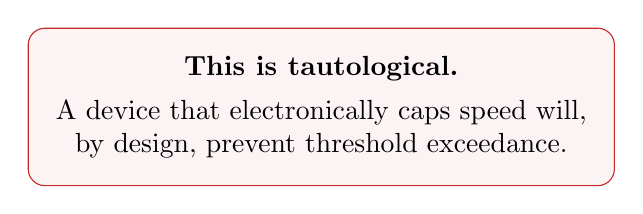
\begin{tikzpicture}
\node[draw=PhaseRed, rounded corners=6pt, fill=PhaseRed!5, inner sep=10pt, font=\normalsize, align=center] {
  \textbf{This is tautological.}\\[4pt]
  A device that electronically caps speed will,\\by design, prevent threshold exceedance.
};
\end{tikzpicture}
\end{center}

\vspace{0.3cm}
\begin{center}
\Large\color{AccentGreen}
\textbf{The right question:}\\[4pt]
\normalsize What happens on the \textbf{unconstrained} behavioral margins?
\end{center}
\end{frame}

% --- Slide: One Lever, Many Margins ---
\begin{frame}{Core Insight: One Lever, Many Margins}
\begin{center}
\begin{tikzpicture}[
  catbox/.style={draw, rounded corners=4pt, minimum width=4.0cm, minimum height=1.6cm, align=center, font=\small, line width=1.2pt},
  scale=0.85, transform shape
  ]
  % Single lever
  \node[catbox, fill=UMNMaroon!10, draw=UMNMaroon, minimum width=4cm] (lever) at (0, 0) {
    \textbf{\color{UMNMaroon}Speed Governor}\\[3pt]
    Single-dimensional\\intervention\\(caps max speed)
  };
  % Safety
  \node[catbox, fill=PhaseRed!10, draw=PhaseRed] (safety) at (7, 1.8) {
    \textbf{\color{PhaseRed}\faShieldAlt~Safety}\\[3pt]
    Harsh accel/decel\\Speed variability (CV)
  };
  % Demand
  \node[catbox, fill=PhaseBlue!10, draw=PhaseBlue] (demand) at (7, 0) {
    \textbf{\color{PhaseBlue}\faChartLine~Demand}\\[3pt]
    Trip frequency\\Distance, retention
  };
  % Dynamics
  \node[catbox, fill=AccentGreen!10, draw=AccentGreen] (dynamics) at (7, -1.8) {
    \textbf{\color{AccentGreen}\faTachometerAlt~Dynamics}\\[3pt]
    Cruising fraction\\Zero-speed fraction
  };
  % Arrows
  \draw[-{Stealth[length=6pt]}, very thick, PhaseRed] (lever.east) -- (safety.west);
  \draw[-{Stealth[length=6pt]}, very thick, PhaseBlue] (lever.east) -- (demand.west);
  \draw[-{Stealth[length=6pt]}, very thick, AccentGreen] (lever.east) -- (dynamics.west);
  % Question marks
  \node[font=\Large, PhaseRed] at (3.5, 1.8) {?};
  \node[font=\Large, PhaseBlue] at (3.5, 0) {?};
  \node[font=\Large, AccentGreen] at (3.5, -1.8) {?};
\end{tikzpicture}
\end{center}

\vspace{0.2cm}
\begin{center}
\footnotesize\color{gray}
Speed reduction is \textit{mechanical} (manipulation check). These margins are \textit{genuinely behavioral}.
\end{center}
\end{frame}

% --- Slide: Research Questions ---
\begin{frame}{Research Questions}
\begin{center}
\large\color{UMNMaroon}\textbf{Three Questions Beyond Speed}
\end{center}

\vspace{0.3cm}
\begin{enumerate}
\item \textbf{Multi-dimensional profiles:} How do safety, demand, and riding dynamics differ across governed vs.\ ungoverned modes---\textit{beyond} the speed dimension?

\vspace{0.2cm}
\item \textbf{Causal multi-outcome:} When the ungoverned mode is removed (Dec 2023), which behavioral margins respond and which don't?

\vspace{0.2cm}
\item \textbf{Compensation:} Do riders compensate on \textit{any} unconstrained margin? (Peltzman / risk homeostasis test)
\end{enumerate}

\vspace{0.3cm}
\textbf{\color{AccentGreen}Contribution:} First multi-outcome causal evaluation of speed governance across safety, demand, and riding dynamics
\end{frame}

% ============================================================
\section{Data \& Setting}

% --- Slide: The Swing Platform ---
\begin{frame}{The Swing Platform: Three Speed Modes}
\begin{center}
\begin{tikzpicture}[
  modebox/.style={draw, rounded corners=6pt, minimum width=3.5cm, minimum height=1.8cm, align=center, font=\footnotesize, line width=1.2pt},
  scale=0.9, transform shape
  ]
  % TUB
  \node[modebox, fill=PhaseRed!10, draw=PhaseRed] (tub) at (0,0) {
    \textbf{\color{PhaseRed}\faRocket~TUB (Turbo)}\\[3pt]
    No speed governor\\
    Max: uncapped\\
    \textbf{54\% speeding rate}
  };
  % STD
  \node[modebox, fill=PhaseBlue!10, draw=PhaseBlue] (std) at (5,0) {
    \textbf{\color{PhaseBlue}\faTachometerAlt~STD (Standard)}\\[3pt]
    Soft governor\\
    Max: $\sim$25 km/h\\
    \textbf{4.2\% speeding rate}
  };
  % ECO
  \node[modebox, fill=AccentGreen!10, draw=AccentGreen] (eco) at (10,0) {
    \textbf{\color{AccentGreen}\faLeaf~ECO (Economy)}\\[3pt]
    Strict governor\\
    Max: $\sim$20 km/h\\
    \textbf{1.1\% speeding rate}
  };
  % Arrow
  \draw[-{Stealth[length=5pt]}, thick, gray] (tub.east) -- (std.west) node[midway, above, font=\tiny, gray] {governed};
  \draw[-{Stealth[length=5pt]}, thick, gray] (std.east) -- (eco.west) node[midway, above, font=\tiny, gray] {stricter};
  % Bottom label
  \node[font=\footnotesize, color=gray, align=center] at (5, -2) {
    Same hardware, same scooter --- only firmware speed setting differs\\
    \textbf{Ideal within-platform comparison}
  };
\end{tikzpicture}
\end{center}
\end{frame}

% --- Slide: Dataset Overview ---
\begin{frame}{Dataset Overview}
\begin{columns}[T]
\begin{column}{0.55\textwidth}
\small
\textbf{\color{UMNMaroon}Swing E-Scooter GPS Data}
\begin{itemize}
\item \textbf{21M} trips, Feb--Nov 2023
\item \textbf{52 cities} across South Korea
\item \textbf{$\sim$1.8M} unique users
\item Sensor speeds at $\sim$10s intervals
\item Mode choice (TUB/STD/ECO) per trip
\end{itemize}
\vspace{0.15cm}
\textbf{\color{PhaseOrange}Additional Variables}
\begin{itemize}
\item Road class (OSM + KDTree)
\item City aggregates, time of day, distance
\item User demographics (age)
\end{itemize}
\end{column}
\begin{column}{0.42\textwidth}
\centering
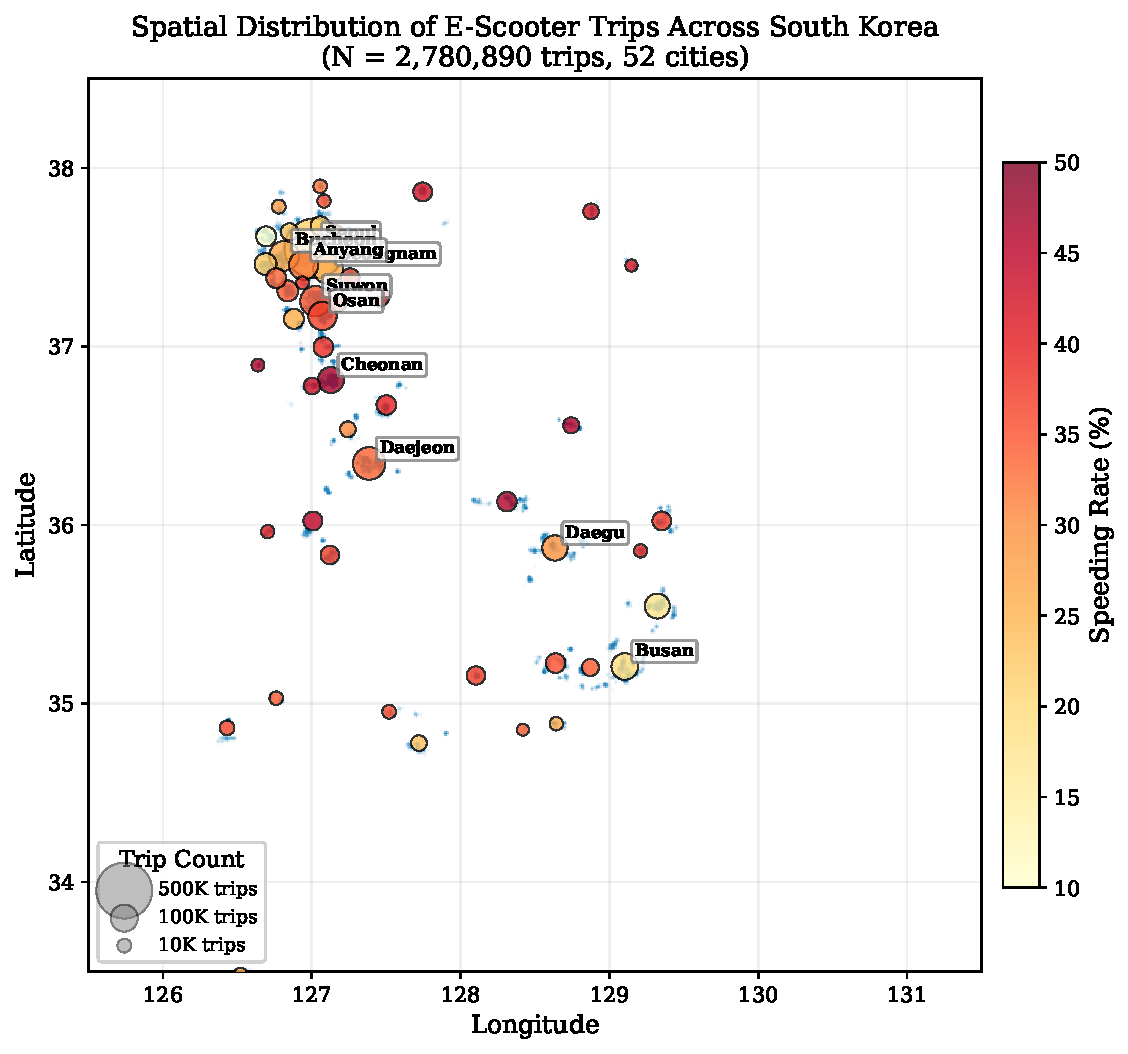
\includegraphics[width=\textwidth,height=0.55\textheight,keepaspectratio]{fig1_spatial_distribution.pdf}
{\footnotesize\color{gray} Trip distribution across Korea}
\end{column}
\end{columns}
\end{frame}

% --- Slide: The Natural Experiment ---
\begin{frame}{The Natural Experiment: December 2023 TUB Ban}
\begin{center}
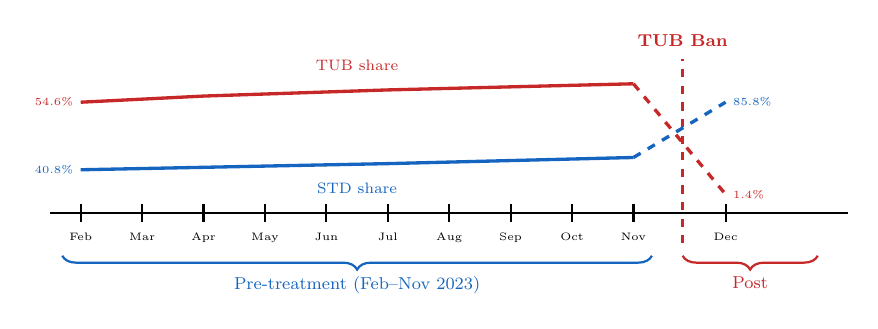
\begin{tikzpicture}[scale=0.78, transform shape]
  % Timeline
  \draw[thick, -] (0,0) -- (13,0);
  % Months
  \foreach \x/\m in {0.5/Feb, 1.5/Mar, 2.5/Apr, 3.5/May, 4.5/Jun, 5.5/Jul, 6.5/Aug, 7.5/Sep, 8.5/Oct, 9.5/Nov, 11/Dec} {
    \draw[thick] (\x, -0.15) -- (\x, 0.15);
    \node[font=\tiny, below] at (\x, -0.2) {\m};
  }
  % Pre-period bracket
  \draw[decorate, decoration={brace, amplitude=5pt, mirror}, thick, PhaseBlue]
    (0.2, -0.7) -- (9.8, -0.7) node[midway, below=6pt, font=\footnotesize, PhaseBlue] {Pre-treatment (Feb--Nov 2023)};
  % Post-period bracket
  \draw[decorate, decoration={brace, amplitude=5pt, mirror}, thick, PhaseRed]
    (10.3, -0.7) -- (12.5, -0.7) node[midway, below=6pt, font=\footnotesize, PhaseRed] {Post};
  % Event marker
  \draw[very thick, PhaseRed, dashed] (10.3, -0.5) -- (10.3, 2.5);
  \node[font=\footnotesize, PhaseRed, align=center, fill=white] at (10.3, 2.8) {\textbf{TUB Ban}};
  % TUB share line (stylized)
  \draw[very thick, PhaseRed] (0.5, 1.8) -- (2.5, 1.9) -- (5.5, 2.0) -- (9.5, 2.1);
  \draw[very thick, PhaseRed, dashed] (9.5, 2.1) -- (11, 0.3);
  \node[font=\tiny, PhaseRed, right] at (11, 0.3) {1.4\%};
  \node[font=\tiny, PhaseRed, left] at (0.5, 1.8) {54.6\%};
  \node[font=\scriptsize, PhaseRed] at (5, 2.4) {TUB share};
  % STD share line
  \draw[very thick, PhaseBlue] (0.5, 0.7) -- (5.5, 0.8) -- (9.5, 0.9);
  \draw[very thick, PhaseBlue, dashed] (9.5, 0.9) -- (11, 1.8);
  \node[font=\tiny, PhaseBlue, right] at (11, 1.8) {85.8\%};
  \node[font=\tiny, PhaseBlue, left] at (0.5, 0.7) {40.8\%};
  \node[font=\scriptsize, PhaseBlue] at (5, 0.4) {STD share};
\end{tikzpicture}
\end{center}

\vspace{0.2cm}
\begin{columns}[T]
\begin{column}{0.48\textwidth}
\footnotesize
\textbf{What happened:} Swing removed TUB mode system-wide in Dec 2023 (regulatory pressure)
\end{column}
\begin{column}{0.48\textwidth}
\footnotesize
\textbf{Why it matters:} Exogenous shock $\to$ multi-outcome causal identification via DiD
\end{column}
\end{columns}
\end{frame}

% ============================================================
\section{Multi-Outcome Framework}

% --- Slide: Outcome Variables ---
\begin{frame}{Outcome Variables: Genuinely Behavioral vs.\ Mechanical}
\small
\begin{columns}[T]
\begin{column}{0.55\textwidth}
\textbf{\color{AccentGreen}Primary Outcomes (genuinely behavioral)}
\vspace{0.1cm}

\textbf{\color{PhaseRed}\faShieldAlt~Safety}
\begin{itemize}
\item Harsh acceleration count
\item Harsh deceleration count
\item Speed CV (within-trip variability)
\end{itemize}

\textbf{\color{PhaseBlue}\faChartLine~Demand}
\begin{itemize}
\item Trip frequency (per user/month)
\item Trip distance (km)
\item User retention / churn
\end{itemize}

\textbf{\color{AccentGreen}\faTachometerAlt~Dynamics}
\begin{itemize}
\item Cruising fraction (\% steady speed)
\item Zero-speed fraction (\% stopped)
\end{itemize}
\end{column}
\begin{column}{0.42\textwidth}
\textbf{\color{gray}Manipulation Check (mechanical)}
\begin{itemize}
\item[\color{gray}\faCheck] Mean speed
\item[\color{gray}\faCheck] Max speed
\item[\color{gray}\faCheck] P85 speed
\end{itemize}
{\footnotesize\color{gray} Reported briefly to confirm the governor works. Not a ``finding.''}

\vspace{0.4cm}
\textbf{\color{PhaseRed}Dropped (artifacts)}
\begin{itemize}
\item[\color{PhaseRed}\faTimes] Speed std (range shrinks mechanically)
\item[\color{PhaseRed}\faTimes] Skewness, kurtosis (truncation)
\end{itemize}
\end{column}
\end{columns}
\end{frame}

% --- Slide: Data Plan ---
\begin{frame}{Unified Data Plan}
\small
\begin{table}
\centering
\begin{tabular}{@{}llll@{}}
\toprule
\textbf{Analysis} & \textbf{Period} & \textbf{N} & \textbf{Unit} \\
\midrule
\rowcolor{PhaseBlue!8}
Cross-sectional (Block 1, 4) & Feb--Nov 2023 & $\sim$21M trips & Trip \\
\rowcolor{PhaseOrange!8}
Multi-outcome DiD (Block 2) & Feb--Dec 2023 & 53$\times$12 panel & City-month \\
\rowcolor{PhasePurple!8}
Compensation test (Block 3) & Nov--Dec 2023 & $\sim$240K users & User \\
\rowcolor{AccentGreen!8}
Escalation/Survival (Block 4) & Feb--Nov 2023 & $\sim$864K users & User \\
\bottomrule
\end{tabular}
\end{table}

\vspace{0.3cm}
\begin{center}
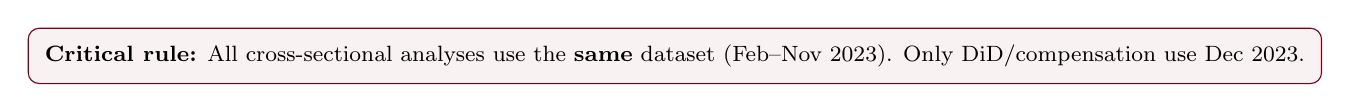
\begin{tikzpicture}
\node[draw=UMNMaroon, rounded corners=4pt, fill=UMNMaroon!5, inner sep=6pt, font=\footnotesize] {
  \textbf{Critical rule:} All cross-sectional analyses use the \textbf{same} dataset (Feb--Nov 2023).
  Only DiD/compensation use Dec 2023.
};
\end{tikzpicture}
\end{center}
\end{frame}

% ============================================================
\section{Block 1: Behavioral Profiles}

% --- Slide: Cross-Sectional ---
\begin{frame}{Block 1: Cross-Sectional Behavioral Profiles}
\textbf{\color{UMNMaroon}Question:} How do safety, demand, and dynamics differ across modes---beyond speed?

\vspace{0.3cm}
\begin{columns}[T]
\begin{column}{0.48\textwidth}
\textbf{Methods}
\begin{itemize}
\item GEE per outcome, clustered by user
\item Within-subject paired comparison (12K multi-mode users, Cohen's $d$)
\item LightGBM + SHAP per outcome category
\end{itemize}
\end{column}
\begin{column}{0.48\textwidth}
\textbf{Key Outputs}
\begin{itemize}
\item Multi-dimensional profiles (radar/parallel coordinates)
\item Forest plot: GEE coefficients across all 8 outcomes
\item SHAP importance comparison across categories
\end{itemize}
\end{column}
\end{columns}

\vspace{0.3cm}
\begin{center}
\footnotesize\color{gray}
v1 results (May only): TUB OR=121 for speeding, SHAP=2.33 (3.6$\times$ next feature).\\
v2 extends to all 8 outcomes on full Feb--Nov dataset.
\end{center}
\end{frame}

% ============================================================
\section{Block 2: Causal Multi-Outcome DiD}

% --- Slide: DiD Design ---
\begin{frame}{Block 2: Multi-Outcome Causal DiD}
\textbf{\color{UMNMaroon}Question:} Which behavioral margins causally respond to removing the ungoverned mode?

\vspace{0.2cm}
\begin{columns}[T]
\begin{column}{0.55\textwidth}
\textbf{TWFE Specification (per outcome)}
\begin{itemize}
\item $Y_{ct} = \alpha_c + \gamma_t + \beta(\text{Post}_t \times \text{TUB}_{c,\text{Nov}}) + \epsilon_{ct}$
\item \textbf{8 primary outcomes} + manipulation check
\item Bonferroni correction for multiple testing
\item City FE + Month FE
\end{itemize}

\vspace{0.2cm}
\textbf{\color{PhaseBlue}NEW: Demand-side outcomes}
\begin{itemize}
\item Trip count per city-month
\item Active user count per city-month
\end{itemize}
\end{column}
\begin{column}{0.42\textwidth}
\centering
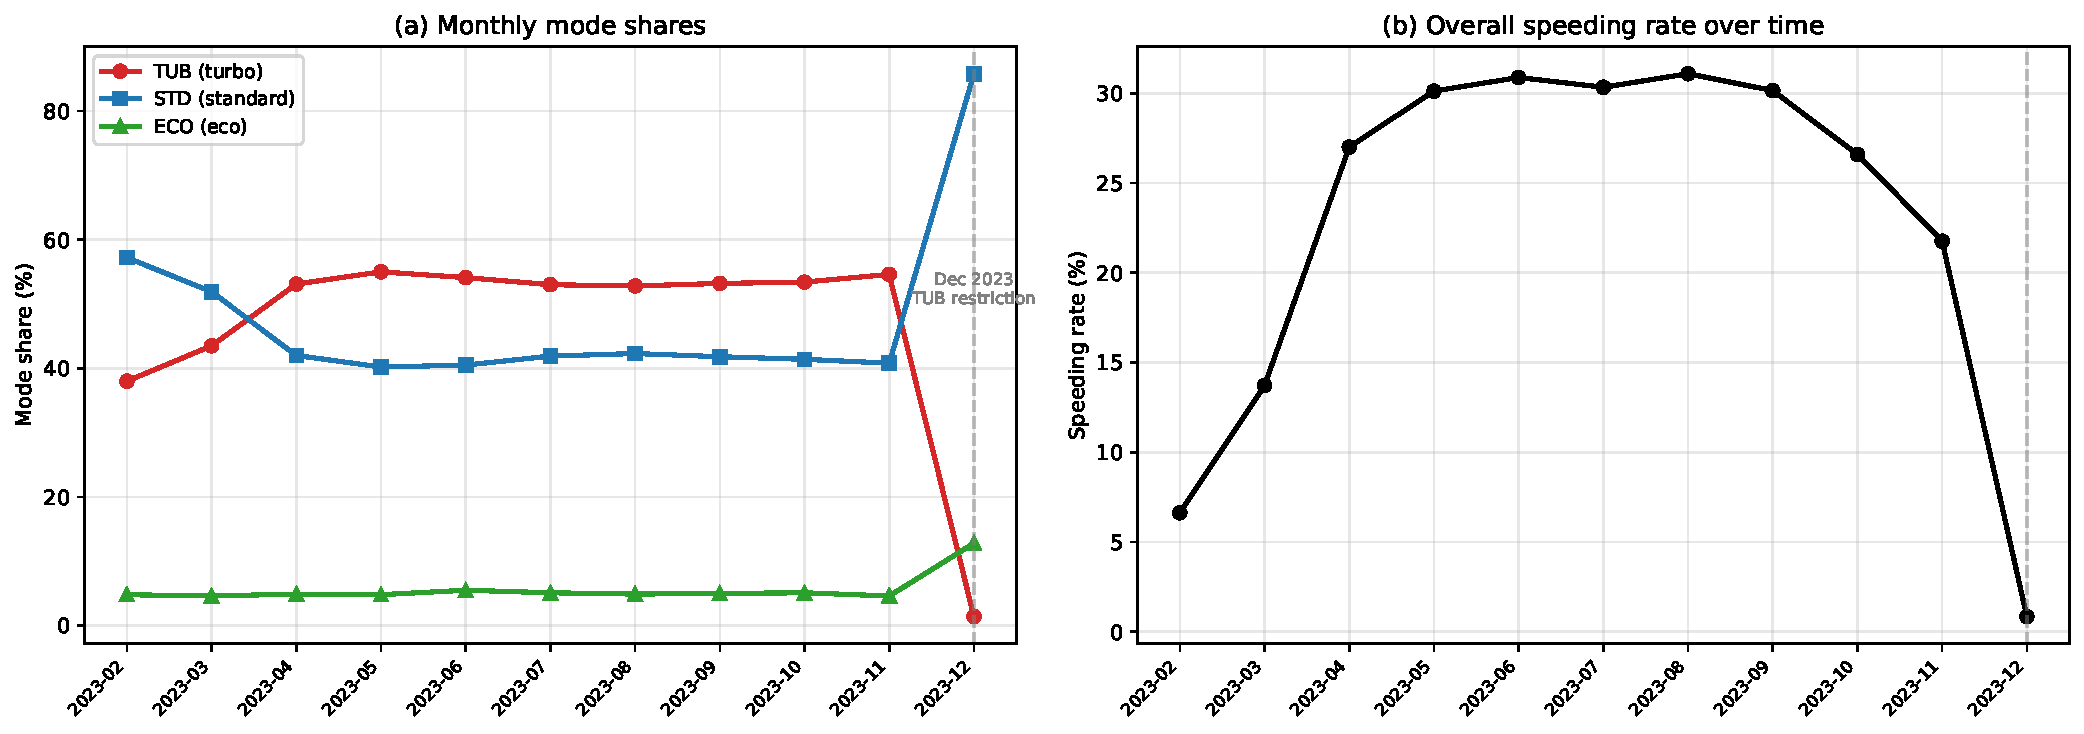
\includegraphics[width=\textwidth,height=0.5\textheight,keepaspectratio]{fig_did_mode_trends.pdf}
{\footnotesize\color{gray} Mode trends around TUB ban}

\vspace{0.15cm}
{\footnotesize v1: $\beta$=--0.568 for speeding.\\v2: extends to all 8 margins.}
\end{column}
\end{columns}
\end{frame}

% --- Slide: KEY FIGURE concept ---
\begin{frame}{The Key Figure: Which Margins Respond?}
\begin{center}
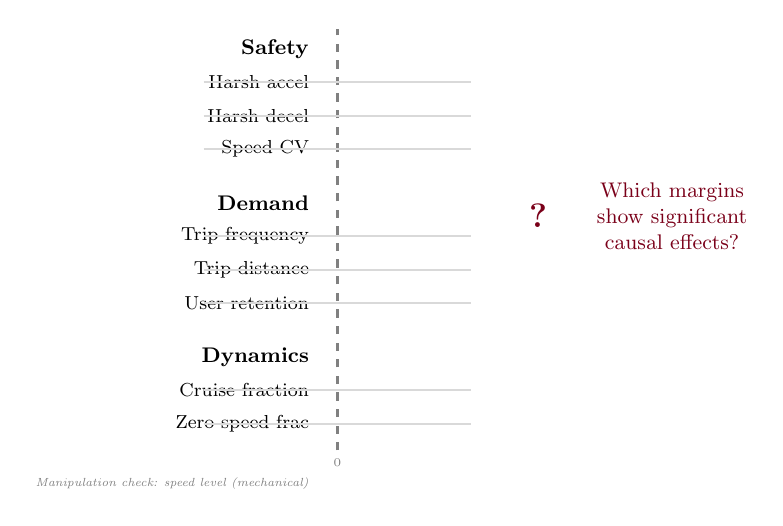
\begin{tikzpicture}[scale=0.85, transform shape]
  % Y-axis labels
  \node[font=\small, anchor=east] at (-0.3, 4.5) {\textbf{Safety}};
  \node[font=\footnotesize, anchor=east] at (-0.3, 4.0) {Harsh accel};
  \node[font=\footnotesize, anchor=east] at (-0.3, 3.5) {Harsh decel};
  \node[font=\footnotesize, anchor=east] at (-0.3, 3.0) {Speed CV};
  \node[font=\small, anchor=east] at (-0.3, 2.2) {\textbf{Demand}};
  \node[font=\footnotesize, anchor=east] at (-0.3, 1.7) {Trip frequency};
  \node[font=\footnotesize, anchor=east] at (-0.3, 1.2) {Trip distance};
  \node[font=\footnotesize, anchor=east] at (-0.3, 0.7) {User retention};
  \node[font=\small, anchor=east] at (-0.3, -0.1) {\textbf{Dynamics}};
  \node[font=\footnotesize, anchor=east] at (-0.3, -0.6) {Cruise fraction};
  \node[font=\footnotesize, anchor=east] at (-0.3, -1.1) {Zero-speed frac};
  % Zero line
  \draw[thick, gray, dashed] (0, -1.5) -- (0, 4.8);
  \node[font=\tiny, gray, below] at (0, -1.5) {0};
  % Conceptual coefficient dots + CI lines (placeholder)
  \foreach \y in {4.0, 3.5, 3.0, 1.7, 1.2, 0.7, -0.6, -1.1} {
    \draw[thick, gray!30] (-2, \y) -- (2, \y);
  }
  % Question marks
  \node[font=\Large, UMNMaroon] at (3, 2) {\textbf{?}};
  \node[font=\small, UMNMaroon, align=center] at (5, 2) {Which margins\\show significant\\causal effects?};
  % Manipulation check (grayed out)
  \node[font=\tiny, gray, anchor=east] at (-0.3, -2.0) {\textit{Manipulation check: speed level (mechanical)}};
\end{tikzpicture}
\end{center}

\vspace{0.1cm}
\begin{center}
\footnotesize
Multi-outcome DiD coefficient plot --- \textbf{the central figure} of the paper.\\
Shows which behavioral margins respond to governance and which are unaffected.
\end{center}
\end{frame}

% ============================================================
\section{Block 3: Compensation Test}

% --- Slide: Compensation ---
\begin{frame}{Block 3: Do Riders Compensate on Any Margin?}
\textbf{\color{UMNMaroon}Peltzman / Risk Homeostasis Test}

\vspace{0.2cm}
\begin{columns}[T]
\begin{column}{0.48\textwidth}
\textbf{Theory (Peltzman 1975)}
\begin{itemize}
\item Safety interventions constrain one margin
\item Agents may compensate on unconstrained margins
\item E.g., seatbelts $\to$ more aggressive driving
\item E.g., helmet laws $\to$ less cycling (demand)
\end{itemize}

\vspace{0.15cm}
\textbf{Our Test}
\begin{itemize}
\item 120K mode-switchers vs 120K never-TUB
\item Within-user DiD on \textbf{all 8 outcomes}
\item Cohen's $d$ across all margins
\item Placebo validation (Oct 2023)
\end{itemize}
\end{column}
\begin{column}{0.48\textwidth}
\textbf{Possible Findings}
\vspace{0.1cm}

\textbf{\color{AccentGreen}If no compensation:}\\
Governors are ``free'' interventions---reduce speed without behavioral side effects.\\[6pt]

\textbf{\color{PhaseRed}If compensation exists:}\\
Policymakers must weigh tradeoffs (e.g., governed riders brake harder or take riskier routes).\\[6pt]

\textbf{\color{PhaseBlue}If demand drops:}\\
Governance has a mobility cost---riders leave the platform or take fewer trips.

\vspace{0.2cm}
{\footnotesize\color{gray} v1 result: $d$=0.069 for speed (negligible).\\v2 extends to all 8 margins.}
\end{column}
\end{columns}
\end{frame}

% ============================================================
\section{Block 4: Escalation Pathway}

% --- Slide: Escalation ---
\begin{frame}{Block 4: Behavioral Escalation Pathway}
\textbf{\color{UMNMaroon}Question:} Does ungoverned mode availability create a behavioral escalation pipeline?

\vspace{0.2cm}
\begin{columns}[T]
\begin{column}{0.52\textwidth}
\textbf{Experience $\to$ TUB Adoption $\to$ Outcomes}
\begin{itemize}
\item Speeding: 3.8\% (1st trip) $\to$ 28.0\% (500+)
\item TUB adoption: 11.5\% $\to$ 47.8\% by trip 50
\item Within STD/ECO: speeding \textbf{flat}
\item \textbf{98.4\%} mediated by TUB adoption
\end{itemize}

\vspace{0.2cm}
\textbf{Multi-Endpoint Survival}
\begin{itemize}
\item Time-to-first-harsh-event
\item Time-to-first-high-CV-trip
\item Time-to-first-speeding (legacy)
\item \textbf{NEW}: Time-to-platform-churn
\end{itemize}
\end{column}
\begin{column}{0.45\textwidth}
\centering
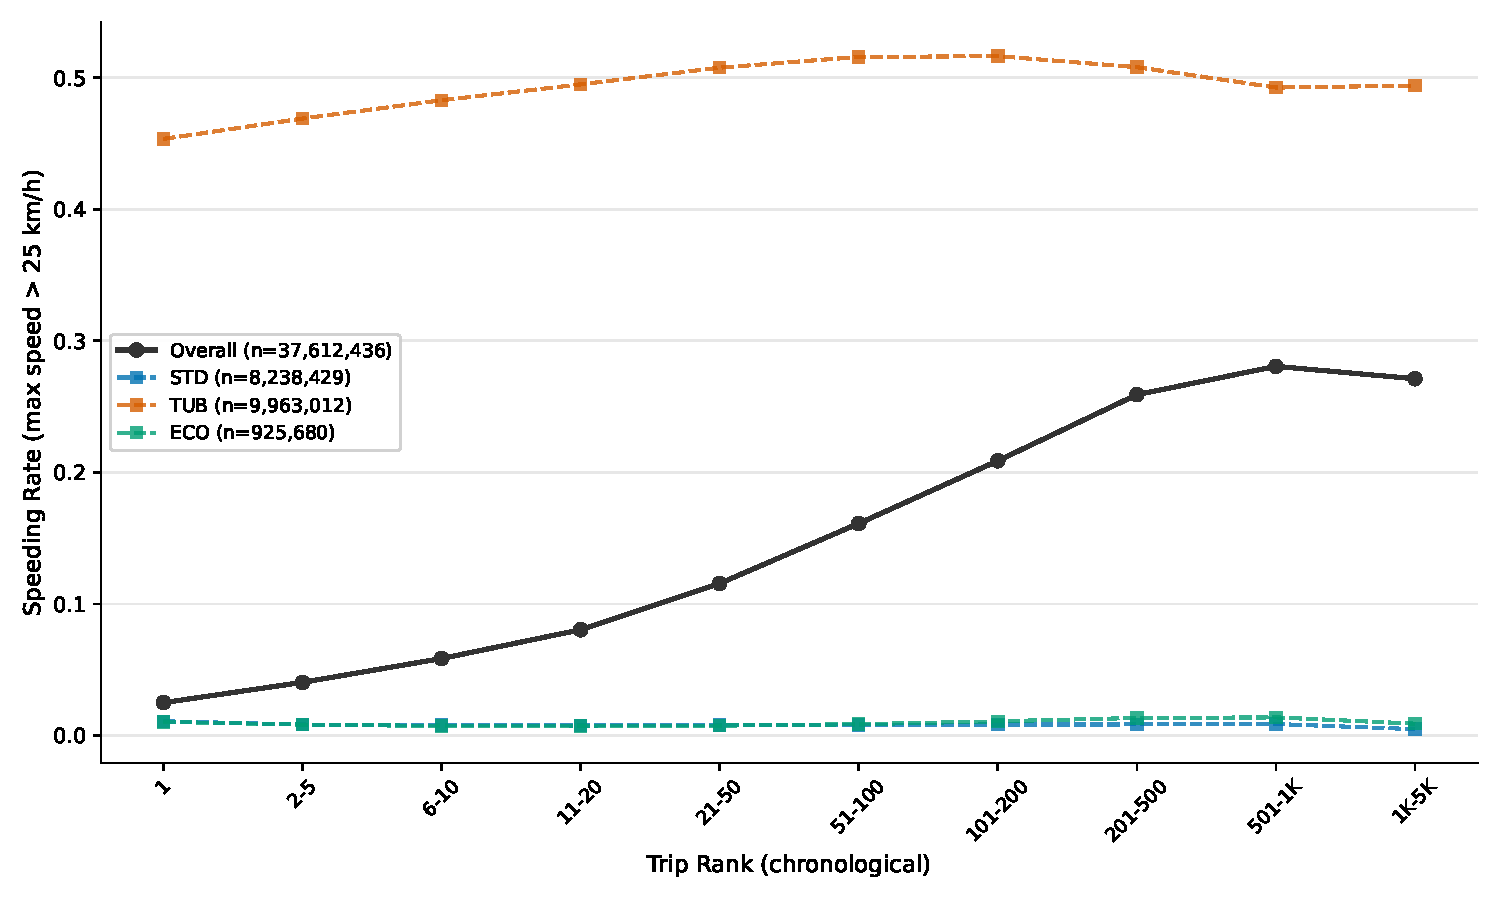
\includegraphics[width=\textwidth,height=0.5\textheight,keepaspectratio]{fig_experience_learning_curve.pdf}
{\footnotesize\color{gray} Experience curve + TUB adoption}

\vspace{0.1cm}
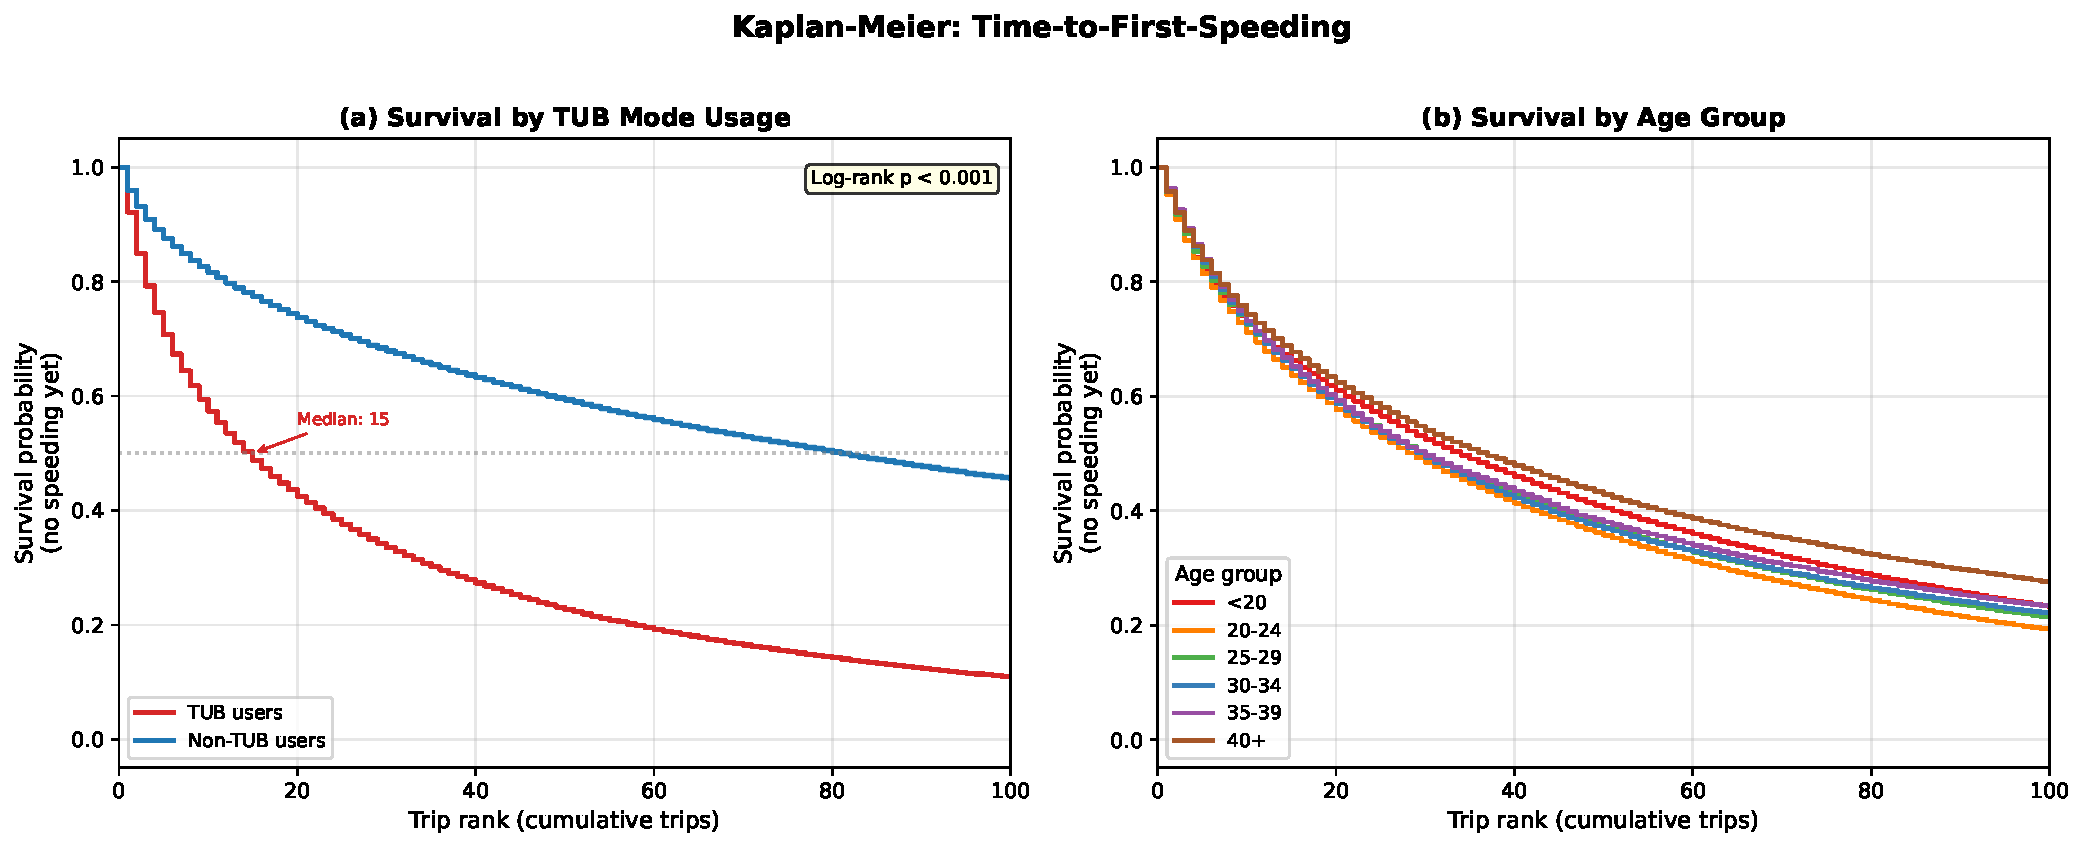
\includegraphics[width=\textwidth,height=0.35\textheight,keepaspectratio]{fig_survival_km.pdf}
{\footnotesize\color{gray} KM curves: TUB vs non-TUB}
\end{column}
\end{columns}
\end{frame}

% ============================================================
\section{Paper Design}

% --- Slide: Candidate Narratives ---
\begin{frame}{Three Candidate Narratives (Decide After Results)}
\begin{center}
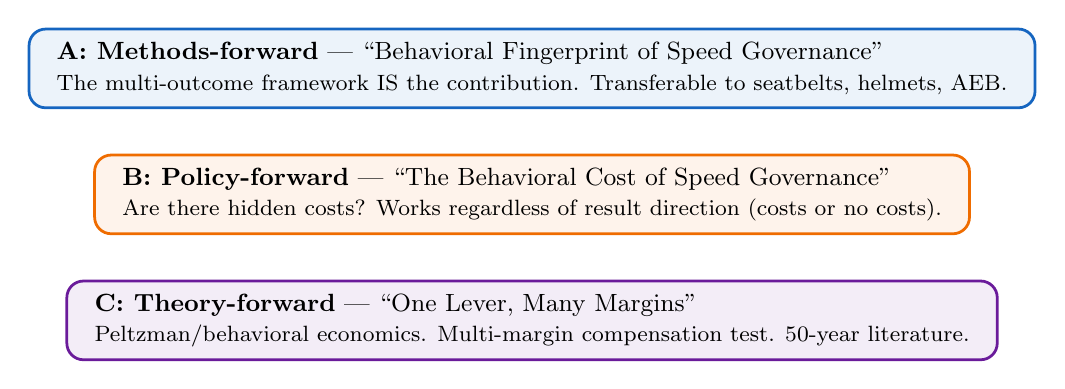
\begin{tikzpicture}[
  narbox/.style={draw, rounded corners=6pt, minimum width=11cm, minimum height=1.0cm, align=left, font=\small, line width=1pt, inner xsep=10pt},
  ]
  \node[narbox, fill=PhaseBlue!8, draw=PhaseBlue] (a) at (0, 2.4) {
    \textbf{A: Methods-forward} --- ``Behavioral Fingerprint of Speed Governance''\\
    \footnotesize The multi-outcome framework IS the contribution. Transferable to seatbelts, helmets, AEB.
  };
  \node[narbox, fill=PhaseOrange!8, draw=PhaseOrange] (b) at (0, 0.8) {
    \textbf{B: Policy-forward} --- ``The Behavioral Cost of Speed Governance''\\
    \footnotesize Are there hidden costs? Works regardless of result direction (costs or no costs).
  };
  \node[narbox, fill=PhasePurple!8, draw=PhasePurple] (c) at (0, -0.8) {
    \textbf{C: Theory-forward} --- ``One Lever, Many Margins''\\
    \footnotesize Peltzman/behavioral economics. Multi-margin compensation test. 50-year literature.
  };
\end{tikzpicture}
\end{center}

\vspace{0.3cm}
\begin{center}
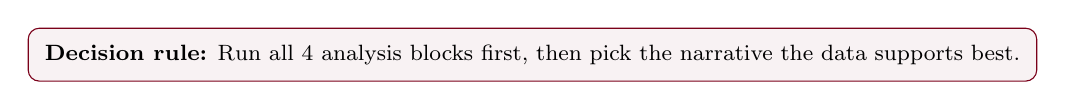
\begin{tikzpicture}
\node[draw=UMNMaroon, rounded corners=4pt, fill=UMNMaroon!5, inner sep=6pt, font=\footnotesize] {
  \textbf{Decision rule:} Run all 4 analysis blocks first, then pick the narrative the data supports best.
};
\end{tikzpicture}
\end{center}
\end{frame}

% --- Slide: Paper Structure ---
\begin{frame}{Paper Structure ($\sim$8,000--10,000 words)}
\footnotesize
\begin{columns}[T]
\begin{column}{0.48\textwidth}
\begin{enumerate}
\item \textbf{Introduction} ($\sim$800 w) --- Tautology problem, right questions, gap
\item \textbf{Background} ($\sim$1,000 w) --- Peltzman, demand elasticity, natural experiments
\item \textbf{Data \& Setting} ($\sim$800 w) --- Swing, 21M trips, TUB ban
\item \textbf{Methods} ($\sim$1,500 w) --- GEE, SHAP, multi-outcome DiD, compensation, survival
\end{enumerate}
\end{column}
\begin{column}{0.48\textwidth}
\begin{enumerate}\setcounter{enumi}{4}
\item \textbf{Results} ($\sim$2,500 w)
  \begin{itemize}\footnotesize
  \item Manipulation check (speed---brief)
  \item Safety margins
  \item Demand margins
  \item Riding dynamics
  \item Compensation test
  \item Escalation pathway
  \end{itemize}
\item \textbf{Discussion} ($\sim$1,000 w) --- Synthesis, policy, Peltzman
\item \textbf{Conclusions} ($\sim$400 w)
\end{enumerate}

\vspace{0.15cm}
\textbf{\color{UMNMaroon}Figures:} 10--12 main + appendix\\
\textbf{Target:} AMAR\\
\textbf{Template:} Elsevier CAS single-column
\end{column}
\end{columns}
\end{frame}

% --- Slide: Figures Plan ---
\begin{frame}{Planned Figures (10--12 Main)}
\small
\begin{columns}[T]
\begin{column}{0.48\textwidth}
\textbf{\color{PhaseBlue}Cross-Sectional (1--3)}
\begin{enumerate}
\item Multi-dimensional profiles by mode
\item GEE coefficients across outcomes
\item SHAP importance by category
\end{enumerate}
\textbf{\color{PhaseOrange}Causal (4--6)}
\begin{enumerate}\setcounter{enumi}{3}
\item \textbf{KEY: Multi-outcome DiD coefficients}
\item Demand response (trips + users)
\item Dose-response across outcomes
\end{enumerate}
\end{column}
\begin{column}{0.48\textwidth}
\textbf{\color{PhasePurple}Compensation (7)}
\begin{enumerate}\setcounter{enumi}{6}
\item Cohen's $d$ across all margins
\end{enumerate}
\textbf{\color{AccentGreen}Escalation (8--9)}
\begin{enumerate}\setcounter{enumi}{7}
\item Experience $\to$ TUB $\to$ mediation
\item Multi-endpoint KM survival
\end{enumerate}
\textbf{\color{gray}Robustness (10)}
\begin{enumerate}\setcounter{enumi}{9}
\item Placebo + heterogeneity panel
\end{enumerate}

{\footnotesize\color{gray}Appendix: event studies, Cox forest, paired details}
\end{column}
\end{columns}
\end{frame}

% --- Slide: What's IN vs OUT ---
\begin{frame}{Scope: What's IN vs OUT}
\small
\begin{columns}[T]
\begin{column}{0.48\textwidth}
\textbf{\color{AccentGreen}\faCheck~IN} {\footnotesize(multi-margin behavioral analysis)}
\begin{itemize}
\item 8 genuinely behavioral outcomes
\item Multi-outcome DiD + Bonferroni
\item \textbf{NEW:} Demand outcomes (trips, retention)
\item Compensation test on all margins
\item Multi-endpoint survival + churn
\item SHAP across outcome categories
\end{itemize}
\end{column}
\begin{column}{0.48\textwidth}
\textbf{\color{PhaseRed}\faTimes~OUT} {\footnotesize(separate papers)}
\begin{itemize}
\item GMM rider typology
\item Curvature risk paradox
\item Road class coefficients
\item Mixed-effects model
\item Two-part hurdle model
\item Multinomial logit
\item Spatial hotspots (mention briefly)
\end{itemize}
\end{column}
\end{columns}
\end{frame}

% ============================================================
\section{Implementation}

% --- Slide: Implementation Phases ---
\begin{frame}{Implementation Phases}
\begin{center}
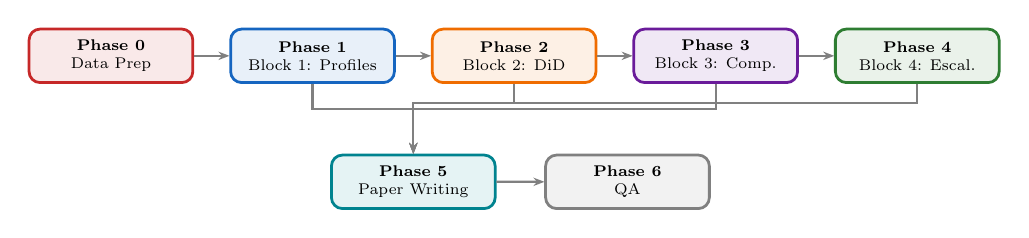
\begin{tikzpicture}[
  phasebox/.style={draw, rounded corners=4pt, minimum width=2.6cm, minimum height=0.85cm, align=center, font=\scriptsize, line width=1pt},
  arrowstyle/.style={-{Stealth[length=4pt]}, thick, gray},
  scale=0.8, transform shape
  ]
  % Phase 0
  \node[phasebox, fill=PhaseRed!10, draw=PhaseRed] (p0) at (0, 0) {\textbf{Phase 0}\\Data Prep};
  % Phase 1
  \node[phasebox, fill=PhaseBlue!10, draw=PhaseBlue] (p1) at (3.2, 0) {\textbf{Phase 1}\\Block 1: Profiles};
  % Phase 2
  \node[phasebox, fill=PhaseOrange!10, draw=PhaseOrange] (p2) at (6.4, 0) {\textbf{Phase 2}\\Block 2: DiD};
  % Phase 3
  \node[phasebox, fill=PhasePurple!10, draw=PhasePurple] (p3) at (9.6, 0) {\textbf{Phase 3}\\Block 3: Comp.};
  % Phase 4
  \node[phasebox, fill=AccentGreen!10, draw=AccentGreen] (p4) at (12.8, 0) {\textbf{Phase 4}\\Block 4: Escal.};
  % Phase 5
  \node[phasebox, fill=PhaseTeal!10, draw=PhaseTeal] (p5) at (4.8, -2) {\textbf{Phase 5}\\Paper Writing};
  % Phase 6
  \node[phasebox, fill=gray!10, draw=gray] (p6) at (8.2, -2) {\textbf{Phase 6}\\QA};
  % Arrows
  \draw[arrowstyle] (p0) -- (p1);
  \draw[arrowstyle] (p1) -- (p2);
  \draw[arrowstyle] (p2) -- (p3);
  \draw[arrowstyle] (p3) -- (p4);
  \draw[arrowstyle] (p1.south) -- ++(0,-0.4) -| (p5.north);
  \draw[arrowstyle] (p2.south) -- ++(0,-0.3) -| (p5.north);
  \draw[arrowstyle] (p3.south) -- ++(0,-0.4) -| (p5.north);
  \draw[arrowstyle] (p4.south) -- ++(0,-0.3) -| (p5.north);
  \draw[arrowstyle] (p5) -- (p6);
\end{tikzpicture}
\end{center}

\vspace{0.2cm}
\footnotesize
\begin{columns}[T]
\begin{column}{0.48\textwidth}
\textbf{Phase 0} builds unified Feb--Nov 2023 dataset with all 8 primary outcomes
\end{column}
\begin{column}{0.48\textwidth}
\textbf{Phase 5} starts after all 4 blocks complete; narrative selected based on results
\end{column}
\end{columns}
\end{frame}

% ============================================================
% SUMMARY
% ============================================================
\begin{frame}{Summary}
\begin{columns}[T]
\begin{column}{0.55\textwidth}
\textbf{\color{UMNMaroon}Core Message}\\
``Does a speed governor reduce speeding?'' is the wrong question. The right question: \textbf{what happens on the unconstrained behavioral margins?}

\vspace{0.3cm}
\textbf{Framework}
\begin{itemize}
\item 8 genuinely behavioral outcomes
\item 3 categories: safety $\times$ demand $\times$ dynamics
\item 4 analysis blocks converging
\item Multi-outcome causal identification
\end{itemize}
\end{column}
\begin{column}{0.42\textwidth}
\textbf{Key Numbers (v1)}
\begin{itemize}
\item 21M trips, 52 cities, 10 months
\item TUB ban: $\beta$=--0.568 (speeding)
\item No compensation: $d$=0.069
\item TUB adoption mediates 98.4\%
\end{itemize}

\vspace{0.2cm}
\textbf{Status}
\begin{itemize}
\item[\color{AccentGreen}\faCheckCircle] v1 analyses (May-only)
\item[\color{PhaseOrange}\faCircle] Re-run on full Feb--Nov
\item[\color{PhaseOrange}\faCircle] Add demand + dynamics outcomes
\item[\color{gray}\faCircle] Write for AMAR
\end{itemize}
\end{column}
\end{columns}
\end{frame}

% ============================================================
% THANK YOU
% ============================================================
\begin{frame}[standout]
\Large Thank you\\[10pt]
\normalsize
\texttt{chois@umn.edu}\\[5pt]
\footnotesize
Seongjin Choi ~|~ University of Minnesota
\end{frame}

% ============================================================
% BACKUP SLIDES
% ============================================================
\appendix

\begin{frame}{Backup: v1 DiD Results}
\small
\begin{columns}[T]
\begin{column}{0.50\textwidth}
\textbf{\color{AccentGreen}Main Results (speeding only)}
\begin{itemize}
\item TWFE: $\beta$ = \textbf{--0.568} ($p < 0.001$)
\item 50\% TUB city $\to$ \textbf{28.4pp} reduction
\item Dose-response: $r$ = \textbf{0.754} (51 cities)
\end{itemize}
\vspace{0.1cm}
\textbf{\color{PhaseBlue}Robustness}
\begin{itemize}
\item Placebo (Sep): $\beta$=--0.015, $p$=0.56 \checkmark
\item Effects in all city-size quartiles
\item Cluster-robust SE ratio = 1.03
\end{itemize}
\end{column}
\begin{column}{0.47\textwidth}
\centering
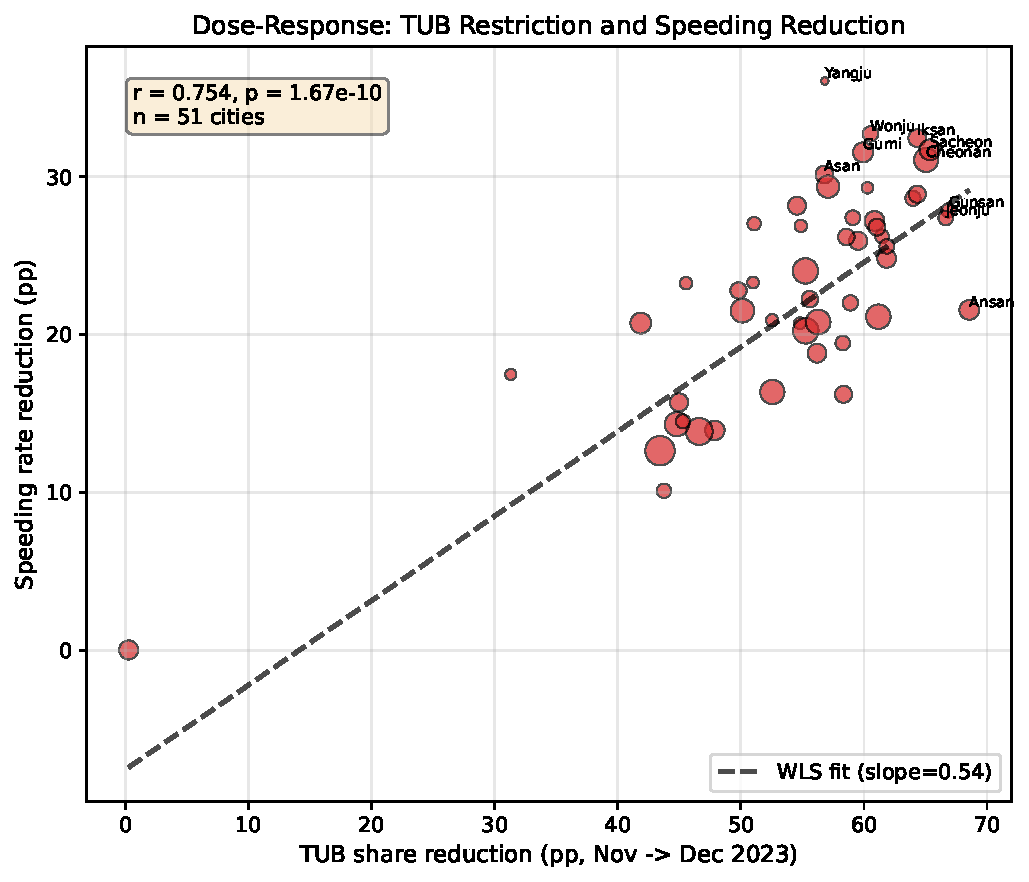
\includegraphics[width=\textwidth,height=0.55\textheight,keepaspectratio]{fig_did_dose_response.pdf}
{\footnotesize\color{gray} Dose-response across cities}
\end{column}
\end{columns}
\end{frame}

\begin{frame}{Backup: v1 Survival Analysis}
\begin{columns}[T]
\begin{column}{0.50\textwidth}
\textbf{Design}
\begin{itemize}
\item 864K users with $\geq$2 trips (Feb--Nov)
\item Event: first trip with max speed $>$ 25 km/h
\item 48\% events, 52\% censored
\end{itemize}

\vspace{0.2cm}
\textbf{Key Findings}
\begin{itemize}
\item KM median: TUB \textbf{15 trips} vs non-TUB \textbf{81 trips}
\item Cox time-varying: TUB adoption \textbf{HR = 10.41}
\item TUB mediates \textbf{98.4\%} of experience-speeding gradient
\end{itemize}
\end{column}
\begin{column}{0.47\textwidth}
\centering
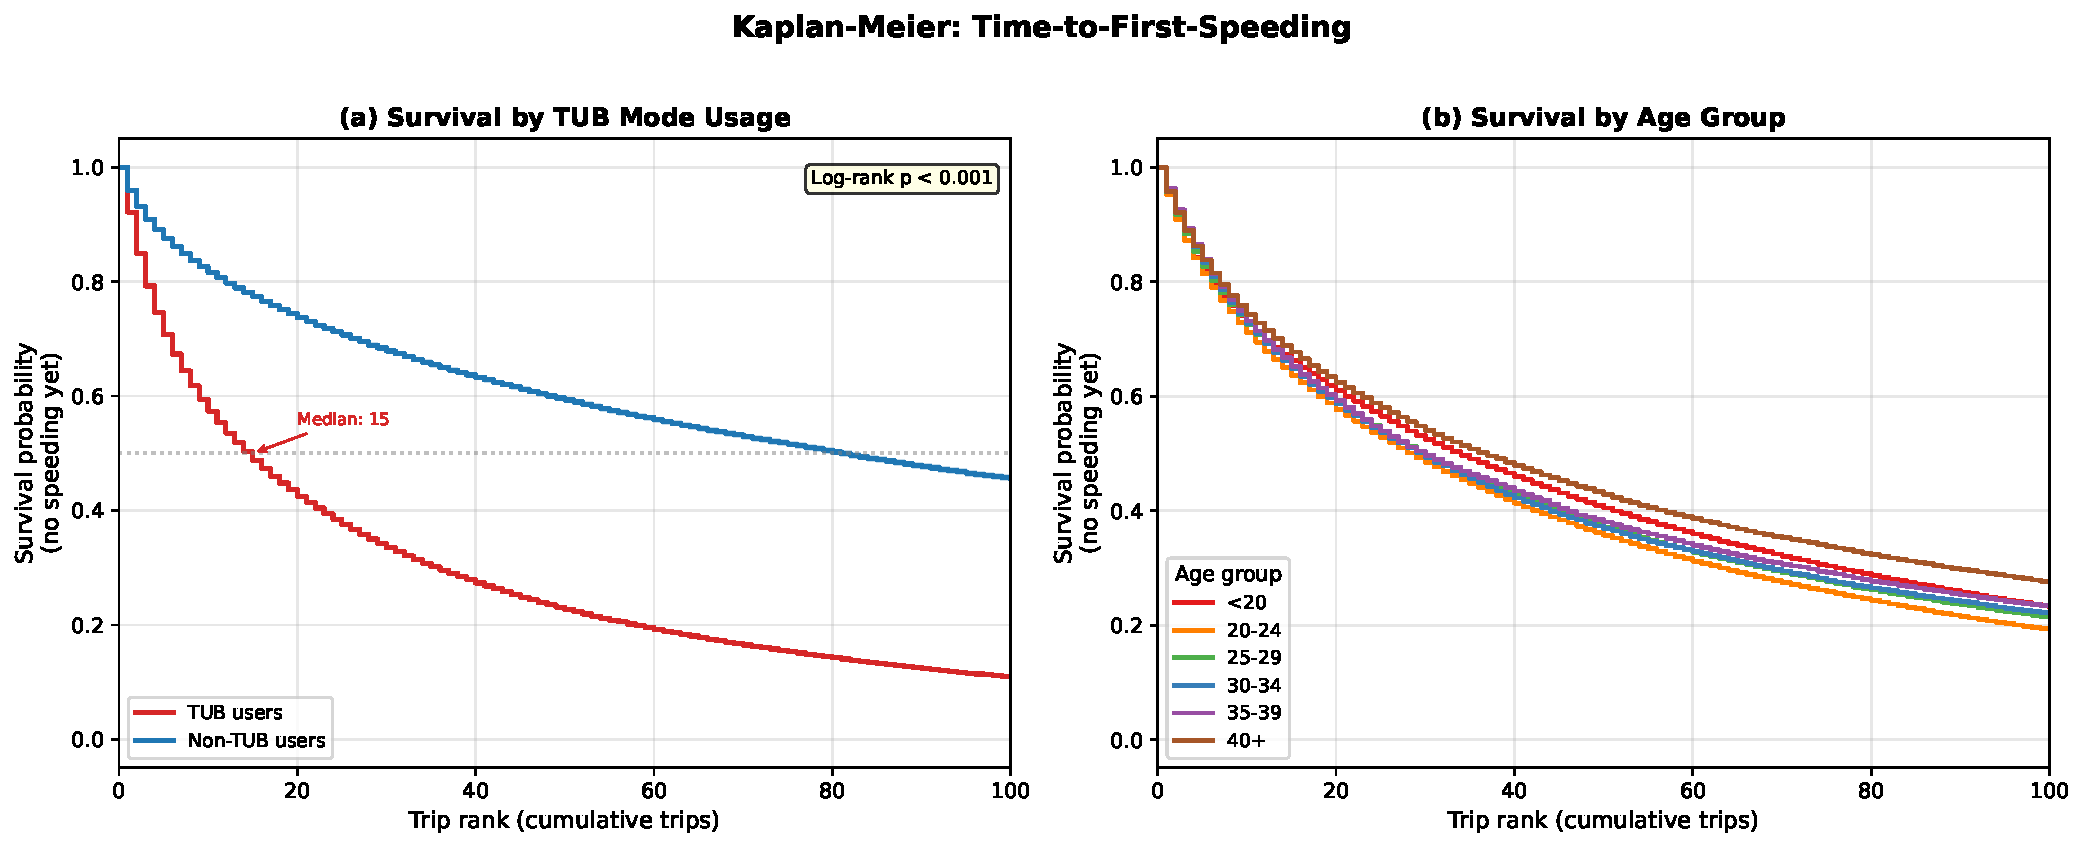
\includegraphics[width=\textwidth,height=0.6\textheight,keepaspectratio]{fig_survival_km.pdf}
{\footnotesize\color{gray} KM curves: TUB vs non-TUB users}
\end{column}
\end{columns}
\end{frame}

\begin{frame}{Backup: v1 Mode-Switcher Analysis}
\begin{columns}[T]
\begin{column}{0.48\textwidth}
\centering
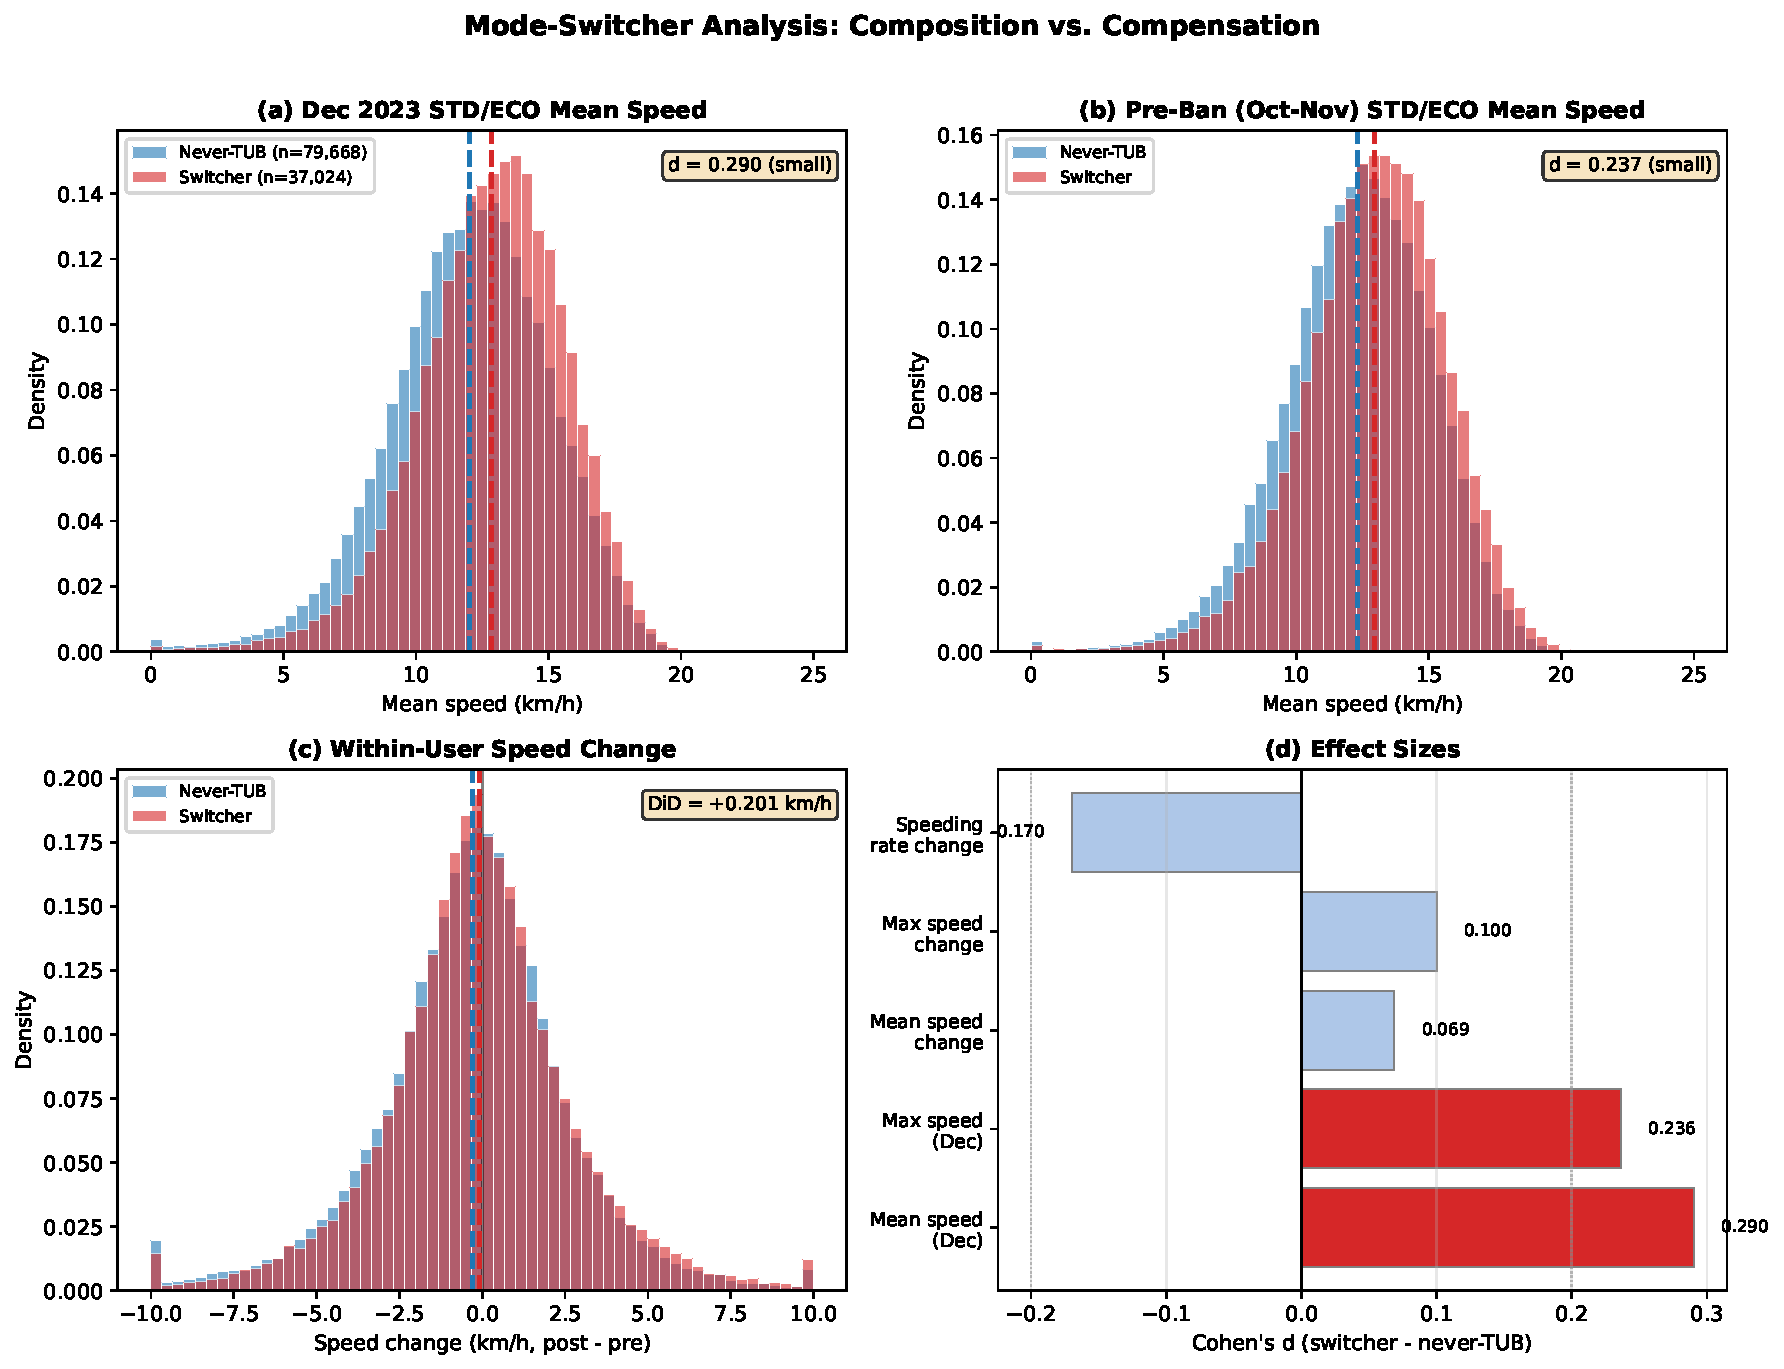
\includegraphics[width=\textwidth,height=0.6\textheight,keepaspectratio]{fig_mode_switcher.pdf}
{\footnotesize Mode-switcher: composition vs compensation}
\end{column}
\begin{column}{0.48\textwidth}
\centering
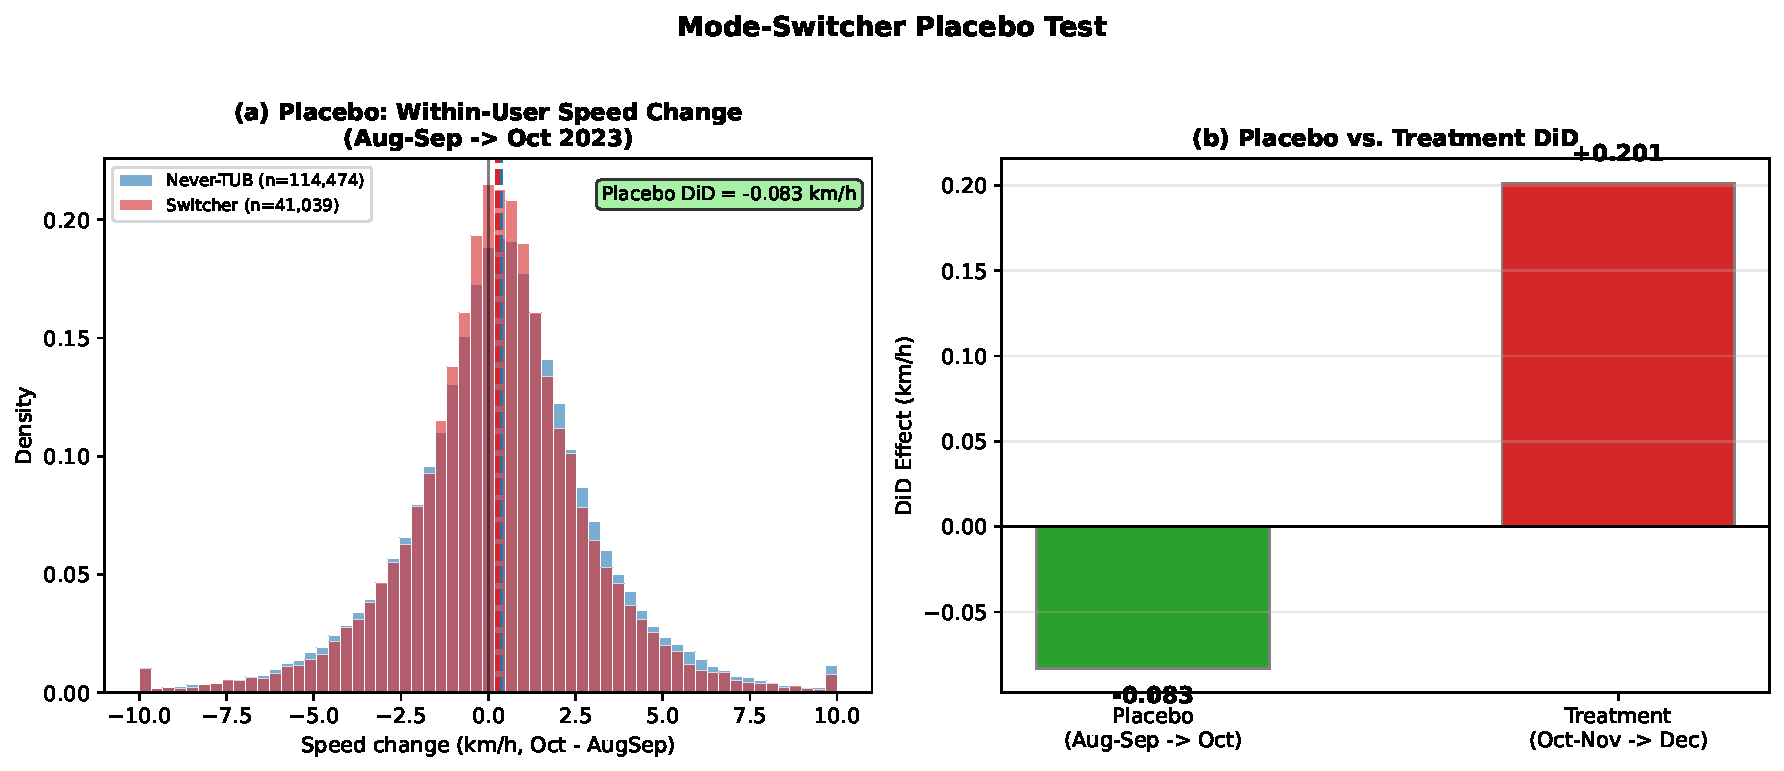
\includegraphics[width=\textwidth,height=0.6\textheight,keepaspectratio]{fig_mode_switcher_placebo.pdf}
{\footnotesize Mode-switcher placebo test}
\end{column}
\end{columns}
\end{frame}

\end{document}
